\documentclass{article}
\usepackage{parskip}
\usepackage{pdfpages}
\usepackage{hyperref}
\usepackage{amsmath}
\usepackage[margin=.6in]{geometry}
\begin{document}
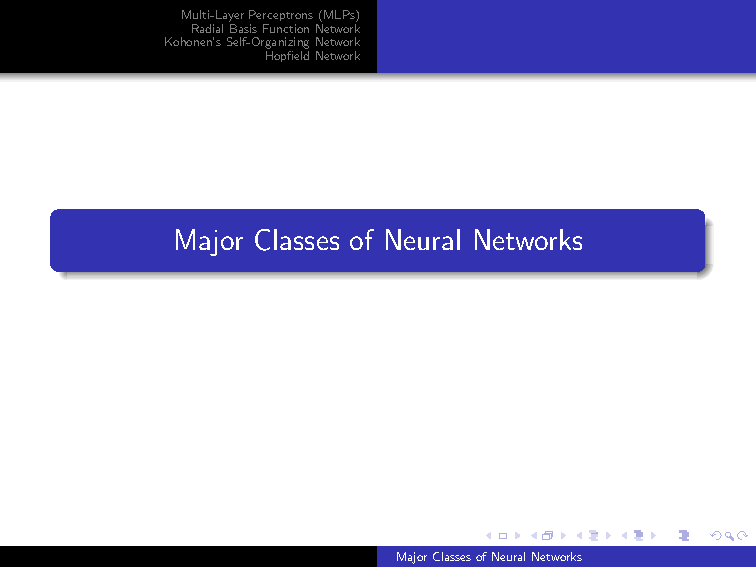
\includepdf[pages=1-6]{slides}
This is the struture of the neural network. It is the most general structure. An input layer is where signals enter the system. These are usually the features of an object. The yellow circles are just units. We call them perceptrons, this is a bit misleading. These perceptrons are different from the ones we saw earlier. The earlier ones create discrete values but they instead (most of the time) they have a smooth, nonlinear activation function. Their activation functions are very differentiable. They have the same structure though. The output layer generates the actual output of the system.

\includepdf[pages=7-9]{slides}
The multilayer perceptron has many layers to propagate signals. Most of the time, these kinds of models are supervised (we have to teach them).

This is still an optimization problem. We have some weights that we want to optimize our weights so that they have the least error. These kinds of systems have a ton of dimensions to optimize across. There will be very complex structures which make it very hard to actually solve. This is why we tend towards using other systems to get an optima even if its not the global optima.

When a solution is found (weights are known) we use this to find the weights of the next layer. This backpropagates the error signal through the layers backwards untill it reaches the first layer. You keep feeling in training signals until you run out and update all the weights. At this point we have finished one epoch.

Say you have $\overrightarrow{x}(x_1, ..., x_m)$ then you have the output $\overrightarrow{y}(y_1, ..., y_l)$ so we then get the mapping $\overrightarrow{y} = f(\overrightarrow{x})$. So your first training signal has to be a bunch of mappings of x to y. Roughly k signals.











\end{document}
